\documentclass{book}

\usepackage{color}

\usepackage{amsmath}
\usepackage{amssymb}
\usepackage{amsthm}

\usepackage{url}

%\usepackage{hyperref}
\usepackage[nottoc,numbib,notlof]{tocbibind}

% For Milnor's Lobachevsy function $\ML$ 
\usepackage[OT2,T1]{fontenc} 
\newcommand{\ML}{\mbox{\fontencoding{OT2}\fontfamily{wncyr}\fontseries{m}\fontshape{n}\selectfont L}} 

\usepackage[a4paper]{geometry}
%\usepackage{fancyhdr}
%\pagestyle{headings}

\setlength{\parindent}{0pt}
\setlength{\parskip}{1ex}

\usepackage{graphicx}
\graphicspath{{image/}{figures/}}

\newtheorem{definition}{Definition}
\newtheorem{proposition}{Proposition}

\newcommand{\R}{\mathbb R}
\newcommand{\C}{\mathbb C}
\newcommand{\Z}{\mathbb Z}
\newcommand{\Chat}{\hat{\mathbb C}}

\title{Uniformization of discrete Riemann surfaces and Applications}
\author{
vorgelegt von\\
Dipl.-Math. techn. Stefan Sechelmann\\
\vspace{0.3cm}\\
von der Fakult{\"a}t II - Mathematik und Naturwissenschaften\\
der Technischen Universit{\"a}t Berlin\\
zur erlangung des akademischen Grades\\
\vspace{0.3cm}\\
Doktor der Naturwissenschaften\\
-- Dr. rer. nat. --\\
\vspace{2cm}\\
Promotionsausschuss\\
\vspace{0.3cm}\\
\begin{tabular}{rl}
Vorsitzender: & NN \\
Gutachter/Berichter: & Prof. Dr. Alexander I. Bobenko \\
& NN 
\end{tabular}
\vspace{0.3cm}\\
Tag der wissenschaftlichen Aussprache: NN\\
\vspace{2cm}\\
}

\date{Berlin, den 07. Januar 2013}

\begin{document}

\frontmatter
\maketitle
\newpage

\tableofcontents
\newpage
\listoffigures

\newpage
\mainmatter
\chapter{Introduction}


\chapter{Discrete Uniformization}

The discrete uniformization theory persented here is based on the notion of discrete conformal eqivalence of triangle meshes. The Euclidean definition was first considered by \cite{Luo2004}, the variational principle and applications in computer graphics is due to \cite{Springborn2008, OWF2009, Bobenko2010}. The notion of conformal equivalence of non-Euclidean metrics and corresponding variational principles were first defined in \cite{Bobenko2010}. \cite{Guo2011} investigate the gradient flow of this principle.
Most of the material presented here can be found in \cite{BobSechSpr}.

\section{Discrete Riemann surfaces}

\begin{figure}
\centering
\scalebox{0.8}{\input{figures/triangles.pdf_t}}
\caption{Discrete surfaces constructed from glued triangles of constant curvature. Euclidean, hyperbolic, and spherical. Bold edegs are identified to create a cone-like singularity at the vertex.}
\label{fig:surface_triangles}
\end{figure}

\begin{definition}
A \emph{discrete surface} is a collection of triangles equipped with a metric of constant Gaussian curvature and geodesic edges. Triangles are glued along edges to form a surface.
\end{definition}

By glueing triangles equipped with a metric of constant Gaussian curvature we obtain a surface that has constant curvature everywhere except for points where the metric has cone-like singularities (Figure~\ref{fig:surface_triangles}). A discrete surface is called Euclidean for $K=0$, hyperbolic for $K=-1$, and spherical if $K=1$.
Remark: In the latter we will use Gaussian curvature and curvature synonymously.
Generically a discrete surface can have boundary components where triangles have not been glued. We consider this case in Section~\ref{sec:planar_domains}. 

A discrete surface consists of vertices, edges, and faces $S=(V, E, F)$. We use single indices for denoting vertices, e.g., $i \in V$. Edges are denoted by $\it{ij}\in E$ and faces $\it{ijk}\in F$.

\begin{definition}
The map $l:E\to \R$ of triangle edge lengths of a discrete surface is called a \emph{discrete Euclidean, hyperbolic, or spherical metric} respectively.
\end{definition}

As in the smooth theory we define what it means for a metric to be conformally eqivalent to another metric. 

\begin{figure}
\centering
\scalebox{0.5}{\input{figures/equivalence.pdf_t}}
\caption{Two Euclidean triangles are discretely conformally equivalent if their edge lengths can be scaled by logarithmic factors $u$ defined on vertices.}
\label{fig:conformal_equivalence}
\end{figure}

\begin{definition}
\label{def:conformal_equivalence_euclidean}
A discrete Euclidean metric with edge lengths $l$ is \emph{discretely conformally equivalent} to the discrete Euclidean metric $\tilde l$ if there is a function $u:V\to \R$ such that for all edges $\it{ij}\in E$ it is
\begin{equation}
l_{\it{ij}} = e^{\frac{1}{2}(u_i + u_j)}\tilde l_{\it{ij}} \label{eq:euclidean_equivalence}
\end{equation}
\end{definition}

This definition is motivated by the smooth theory of Riemann surfaces where two metrics $g$ and $\tilde g$ on a $2$-manifold $M$ are conformally equivalent if there is a smooth function $u:M\to \R$ with \[g=e^{2u}\tilde g.\]

Every Euclidean metric is discretely conformally equivalent to a corresponding hyperbolic or spherical metric by the following \ref{eq:spherical_equivalence}

\begin{definition}
\label{def:conformal_equivalence_general}
A discrete Euclidean metric $l$ and a discrete hyperbolic or discrete spherical metric $\tilde l$ are \emph{discretely conformally equivalent} if for all edges $\it{ij}\in E$
\begin{align}
l_{\it{ij}} &= 2\sinh \frac{\tilde l_{\it{ij}}}{2} \label{eq:hyperbolic_equivalence}\\
l_{\it{ij}} &= 2\sin \frac{\tilde l_{\it{ij}}}{2} \label{eq:spherical_equivalence}
\end{align}
for $\tilde l$ hyperbolic or spherical respectively.
\end{definition}

Literally this means that in the spherical case each triangle can be fit onto the sphere. The conformally equivalent spherical lengths are the lengths of spherical geodesics connecting the triangle vertices. 


\section{Variational principles}

\subsection{Discrete conformal equivalence}

\begin{definition}
	Two Euclidean triangulations $T$ and $\tilde{T}$ are \emph{discretely conformally equivalent} if there is a map $u:V \to \mathbb{R}$ such that for any edge $\it{ij}$ it is
	\[l_{ij}=e^{u_i+u_j}\tilde{l}_{\it{ij}}\]
where $l_{ij}$ is the length of the edge $\it{ij}$.
\end{definition}

\begin{definition}
	A \emph{discrete flat Euclidean metric} is a map $l:E\to\mathbb{R_+}$ such that triangle inequalities are satisfied and angle sums around each inner vertex are equal to $2\pi$. 
\end{definition}


\subsection{Variational principles for discrete metrics in $\mathbb{E}^2$, $\mathbb{H}^2$, and $\mathbb{S}^2$ }
Construction of discrete flat metrics. A discrete Euclidean flat metric is the minimizer of a convex functional.
\begin{eqnarray}
\lambda_{ij} &:=& 2\log l_{ij}\\
\tilde\lambda_{ij} &:=& \lambda_{ij}+u_i+u_j\\
f_{Euc}(u_i, u_j, u_k) &:=& \alpha_i \tilde \lambda_{jk} + \alpha_j \tilde \lambda_{ki} + \alpha_k \tilde \lambda_{ij} + 2\left(\ML(\alpha_i) + \ML(\alpha_j) + \ML(\alpha_k)\right)
\end{eqnarray}

\begin{definition}
\begin{eqnarray}
	E_{Euc}(u) &:=& \sum_{ijk\in F}\left(f_{Euc}(u_i, u_j, u_k) - \frac{\pi}{2}\left(\tilde \lambda_{jk} + \tilde \lambda_{ki} + \tilde \lambda_{ij}\right)\right) + \sum_{i\in V} \Theta_i u_i
\end{eqnarray}
\end{definition}

 This definition and the derivatives can be found in \cite{Bobenko2010}

For the hyperbolic case $\lambda$ and $\tilde\lambda$ are defined as before. Further define
\begin{eqnarray}
	\beta_i &:=& \frac{1}{2} \left(\pi + \alpha_i - \alpha_j - \alpha_k \right)\\
	\beta_j &:=& \frac{1}{2} \left(\pi - \alpha_i + \alpha_j - \alpha_k \right)\\
	\beta_k &:=& \frac{1}{2} \left(\pi - \alpha_i - \alpha_j + \alpha_k \right)\\
	f_{Hyp}(u_i, u_j, u_k) &:=&\beta_i \tilde \lambda_{jk} + \beta_j \tilde \lambda_{ki} + \beta_k \tilde \lambda_{ij}\\ 		
				&&+\ML(\alpha_i) + \ML(\alpha_j) + \ML(\alpha_k) + \ML(\beta_i) + \ML(\beta_j) + \ML(\beta_k)\\
				&&+\ML\left(\frac{1}{2} (\pi - \alpha_i - \alpha_j - \alpha_k)\right)
\end{eqnarray}

\begin{definition}
\begin{eqnarray}
	E_{Hyp}(u) &:=& \sum_{ijk\in F}\left(f_{Hyp}(u_i, u_j, u_k) - \frac{\pi}{2}\left(\tilde \lambda_{jk} + \tilde \lambda_{ki} + \tilde \lambda_{ij}\right)\right) + \sum_{i\in V} \Theta_i u_i
\end{eqnarray}
\end{definition}

\subsection{Realization}


\section{Uniformization of surfaces of higher genus}
Triangulated surfaces of genus $g\geq 2$ without boundary can be equipped with a discretely conformally equivalent flat hyperbolic metric \cite{Bobenko2010}. By flat hyperbolic metric we mean that the edge length are hyperbolic and for any vertex the angle sum is $2\pi$. To realize this metric in the hyperbolic plane e.g. in the Poicar\'e disk model one has to introduce cuts along a basis of the homotopy. This creates a simply connected domain in $\mathbb H^2$. Matching cut paths are realated by a hyperbolic motion i.e. the M\"obius transformations that leave the unit disk invariant (Figure~\ref{fig:axes_of_motion}).

\subsection{The cut-graph and fuchsian groups}
\emph{Want so say here: the number of transformations generated by the mapping of corresponding edges equals the number of path segments in the homotopy-cut-graph. They generate a fuchsian group with \#vertices relations}

\begin{proposition}
	
\end{proposition}

\begin{figure}
\centering
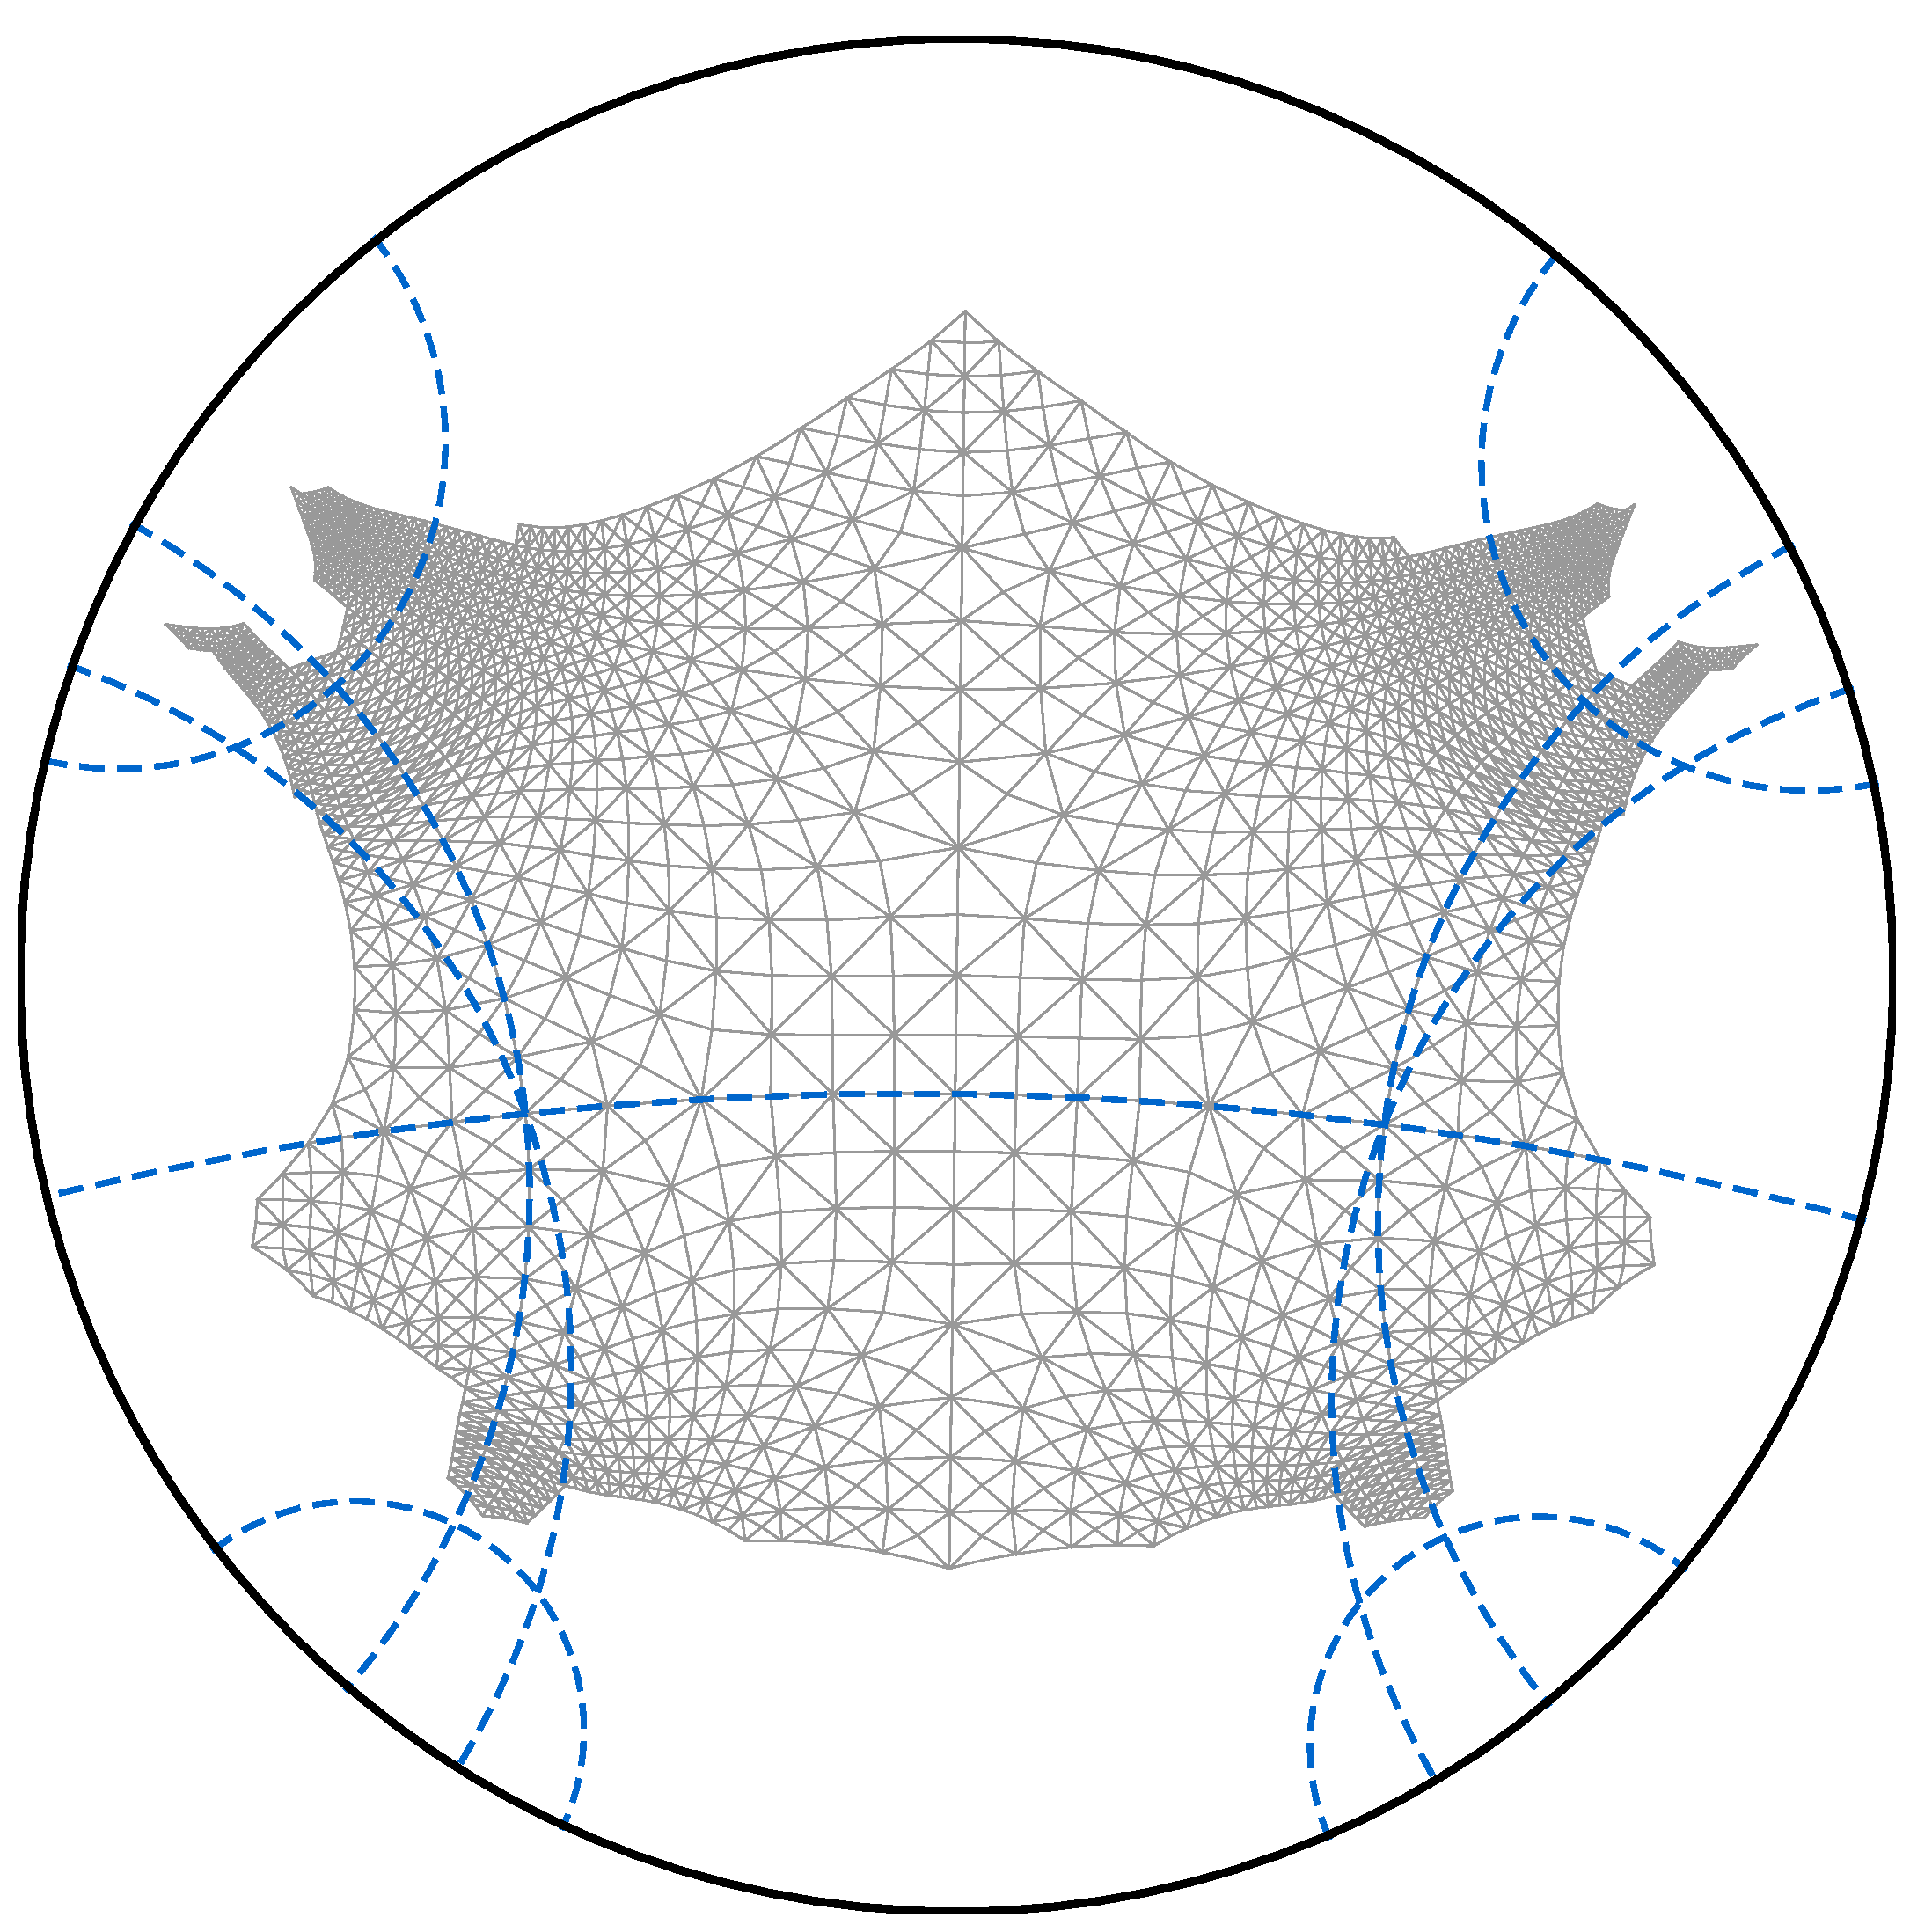
\includegraphics[width=0.4\linewidth]{cutCuttedBrezel01}
\caption{Hyperbolic flat metric on a genus $2$ surface and the axes of the associated hyperbolic motions.}
\label{fig:axes_of_motion}
\end{figure}

\subsection{Minimal presentation}

\section{Canonical fundamental domains of fuchsian groups}
\subsection{Separated handles}
\subsection{Opposite sides identified}

\section{Uniformization of elliptic and hyperelliptic surfaces}
\subsection{Elliptic Functions}
\subsection{The moduli space}
\subsection{Numerical convergence analysis}
\subsection{The modulus of the Wente torus}

\subsection{Construction of hyperelliptic surfaces}
Any hyperelliptic Riemann surface can be expressed as an algebraic curve of the form
\[ w^2 = \prod_{i=1}^{2g+2}(z-\lambda_i) \quad\quad g\geq1,\quad \lambda_i\neq \lambda_j \forall i\neq j.\]
Here $\lambda_i$ are the branch points of the doubly covered Riemann sphere.

\subsection{Weierstrass points on hyperelliptic surfaces}
A hyperelliptic surface comes together with a holomorphic involution $h$ called the hyperelliptic involution. The branch points are fixed points under this transformation. For a hyperelliptic algebraic curve it is $h(\mu, \lambda)=(-\mu, \lambda)$

\subsection{Canonical domains}
\subsection{Lawsons surface}


\section{Meromorphic functions (planned)}
\subsection{Conformal maps to $\hat{\mathbb{C}}$ with singularities}
\subsection{Selection of Branch Data}
\subsection{Examples}

\section{Simply and multiply connected domains}
\label{sec:planar_domains}
\subsection{Variation of edge length}
\subsection{Examples}
\begin{figure}
	\centering
	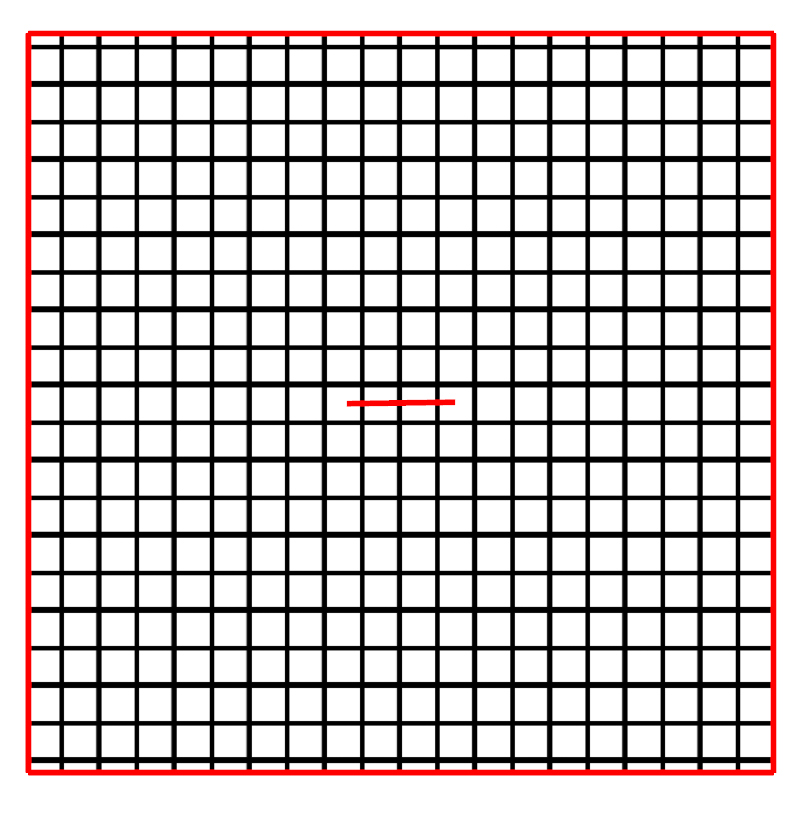
\includegraphics[width=0.3\linewidth]{image/slit_domain/domain_grid.png}
	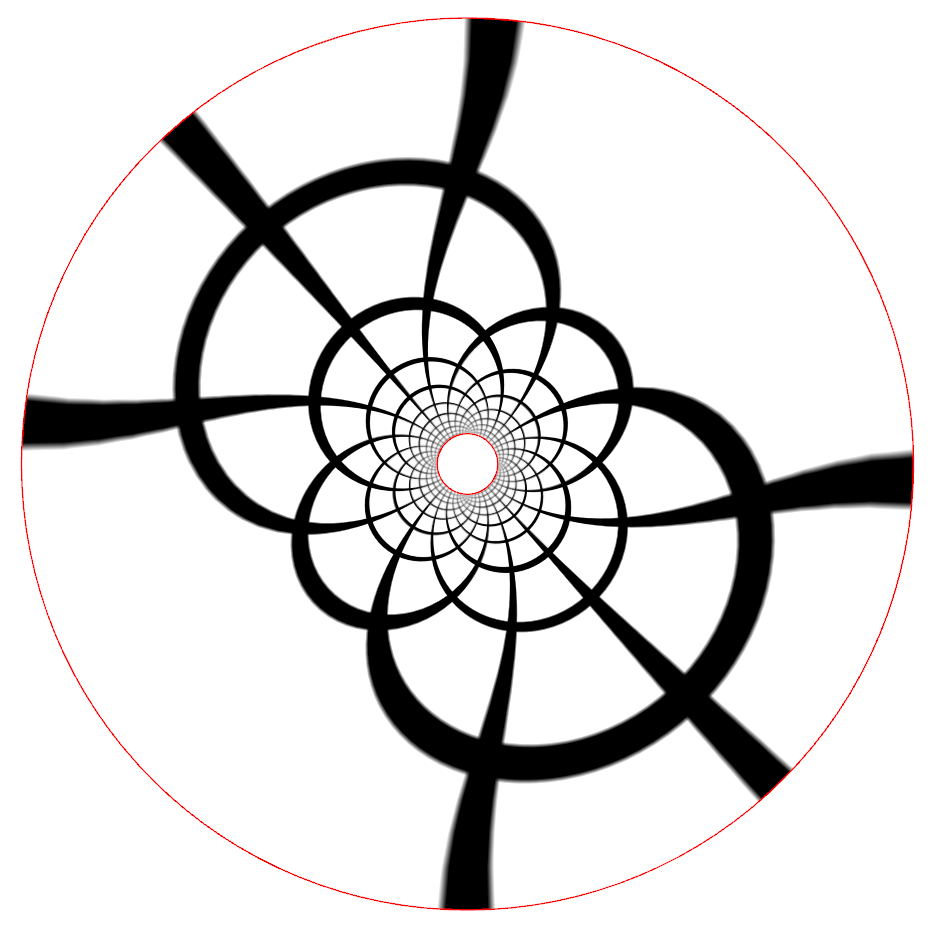
\includegraphics[width=0.3\linewidth]{image/slit_domain/image_grid.png}
	\caption{Square with symmetric slit to the circle}
	\label{fig:slit_circle}
\end{figure}


\section{Conformal maps of planar domains}
\subsection{Boundary conditions}
\subsection{Comparison with examples of the Schwarz-Christoffel community}

\chapter{Discrete Surface Parameterization}


\section{Discrete quasiisothermic parametrizations}
The notion of quasiconformal parameterizations

\subsection{Discrete quasiisothermic parameterizations}

\subsection{Formulation as boundary value problem}
\subsection{Global approach}
\subsection{Variational principle for S-isothermic surfaces}
\subsection{Constructing the associated family of apploximate minimal surfaces}
\subsection{A discrete ellipsoid and its dual surface}
\subsection{Applications in architecture}

\section{Piece-wise projective interpolation for arbitrary parameterizations}
\subsection{Approximation by conformal deformation}
\subsection{Examples}

\section{A variational principle for discrete Tschebyshev nets}
\subsection{Tschebyscheff Meshes}
\subsection{Variational Principle}
\subsection{Applications in architecture}

\newpage
\backmatter 
\bibliographystyle{alpha}
%disable numbering 
\setcounter{secnumdepth}{-1} 
\bibliography{Thesis}

\end{document}





































 